% =====================================================================
% EcoSort — artigo (IEEE Conference, duas colunas)
% Compilar no Overleaf com pdfLaTeX. Enviar também a pasta figuras/.
% Todos os números vêm de resultados/*.json e resultados/*.md do repositório.
% =====================================================================
\documentclass[conference]{IEEEtran}
\usepackage[T1]{fontenc}
\usepackage[utf8]{inputenc}
\usepackage[brazilian]{babel}
\usepackage{graphicx}
\usepackage{booktabs}
\usepackage{amsmath}
\usepackage{url}
\usepackage[hidelinks]{hyperref}
\graphicspath{{figuras/}}

\begin{document}

\title{EcoSort: Integração de Visão Computacional, Processamento de Linguagem Natural e Sistema Baseado em Regras para Orientação ao Descarte de Resíduos}

% >>> PREENCHER: nomes completos dos integrantes <<<
\author{\IEEEauthorblockN{Nome Completo 1, Nome Completo 2, Nome Completo 3, Nome Completo 4}
\IEEEauthorblockA{Curso de \textless curso\textgreater{} --- AFYA / UNIMA, Maceió, AL, Brasil\\
\{email1, email2, email3, email4\}@\textless dominio\textgreater}}

\maketitle

\begin{abstract}
O descarte incorreto de resíduos compromete a coleta seletiva e reduz o reaproveitamento de materiais recicláveis. Este trabalho apresenta o EcoSort, uma aplicação que recebe a foto de um resíduo e uma pergunta livre em português e responde como descartá-lo segundo o padrão brasileiro de cores da coleta seletiva. O sistema integra três componentes em um único fluxo: (i) um classificador de imagens baseado em MobileNetV2 com transfer learning, treinado no dataset TrashNet para seis classes de material; (ii) um reconhecedor de intenções com TF-IDF e Regressão Logística, treinado em um corpus próprio de 335 frases; e (iii) um agente reativo baseado em regras que combina classe, confiança e intenção, consulta uma base de conhecimento e trata explicitamente a incerteza das percepções. No conjunto de teste, o classificador visual obteve acurácia de 86,8\% e F1 macro de 0,846; o modelo de intenções alcançou acurácia de 84,3\%, superando o baseline Naive Bayes (74,5\%). Com limiar de confiança de 0,6, o componente de decisão responde diretamente em 76,3\% das imagens com 96,6\% de acerto e solicita nova foto ou apresenta duas hipóteses nos demais casos. O código é aberto e reprodutível em CPU.
\end{abstract}

\begin{IEEEkeywords}
visão computacional, transfer learning, reconhecimento de intenções, sistemas baseados em regras, coleta seletiva.
\end{IEEEkeywords}

% ---------------------------------------------------------------------
\section{Introdução}
A Política Nacional de Resíduos Sólidos (Lei n.º 12.305/2010) estabelece a coleta seletiva e a responsabilidade compartilhada pelo ciclo de vida dos produtos \cite{pnrs}. Na prática, porém, o cidadão frequentemente tem dúvidas pontuais: em qual lixeira colocar um objeto, se ele é reciclável, se precisa ser lavado ou onde entregá-lo. Erros de separação contaminam lotes recicláveis e aumentam o volume destinado a aterros.

Aplicações de Inteligência Artificial podem reduzir esse atrito: um modelo de visão identifica o material, e uma interface em linguagem natural permite ao usuário perguntar o que deseja saber. Entretanto, classificadores isolados não sabem \emph{o que responder} e erram com frequência não desprezível; um sistema útil precisa decidir o que fazer com percepções incertas.

O objetivo deste trabalho é projetar, implementar e avaliar o EcoSort, cujo público-alvo são cidadãos que separam resíduos em casa, no trabalho ou na universidade. As contribuições são: (1) um fluxo único que integra visão computacional, processamento de linguagem natural (PLN) e um componente de decisão; (2) um corpus de 335 frases em português rotuladas em cinco intenções, com gírias e erros de digitação; (3) um agente baseado em regras que trata a incerteza da visão e do PLN de forma explícita e explicável; e (4) uma avaliação experimental com análise de erros e de limiar de confiança. O código está disponível em \url{https://github.com/FelipeNobreC/ecosort}.

% ---------------------------------------------------------------------
\section{Fundamentação e Trabalhos Relacionados}
\textbf{Classificação de resíduos.} Yang e Thung \cite{trashnet} publicaram o TrashNet, com 2.527 imagens em seis classes (papelão, vidro, metal, papel, plástico e rejeito), e compararam SVM com características SIFT a uma CNN treinada do zero, obtendo 63\% e 22\% de acurácia, respectivamente, o que evidencia a dificuldade de treinar redes profundas com poucos dados.

\textbf{Transfer learning.} Redes pré-treinadas no ImageNet \cite{imagenet} aprendem filtros genéricos reutilizáveis; ajustar apenas as camadas finais a um novo domínio é eficaz com poucos exemplos \cite{yosinski}. A MobileNetV2 \cite{mobilenetv2} usa convoluções separáveis em profundidade e blocos residuais invertidos, com custo computacional adequado à execução em CPU.

\textbf{Reconhecimento de intenções.} Em assistentes conversacionais, a intenção do usuário é tratada como classificação de texto. Representações TF-IDF combinadas a classificadores lineares, como Regressão Logística e Naive Bayes, são baselines fortes para textos curtos e poucos dados \cite{wang2012}.

\textbf{Agentes e sistemas baseados em regras.} Um agente reativo seleciona ações a partir da percepção atual por meio de regras condição--ação \cite{russell}. Sistemas especialistas representam o conhecimento do domínio em uma base separada do motor de inferência, o que facilita manutenção e explicação das decisões.

% ---------------------------------------------------------------------
\section{Metodologia}

\subsection{Arquitetura}
A Fig.~\ref{fig:arq} apresenta o fluxo. O usuário envia a imagem, processada pelo módulo de visão, que retorna a classe mais provável, sua probabilidade (confiança) e as duas classes mais prováveis (top-2). A pergunta é processada pelo módulo de PLN, que retorna a intenção e sua confiança. O módulo de decisão combina essas percepções, consulta a base de conhecimento e produz a resposta, juntamente com a identificação da regra acionada. A interface foi implementada em Streamlit. O ambiente usou Python 3.12, PyTorch 2.15 \cite{pytorch} (versão CPU), torchvision 0.29, scikit-learn 1.9 \cite{sklearn} e seed fixa 42 em todas as etapas aleatórias.

\begin{figure}[t]
\centering
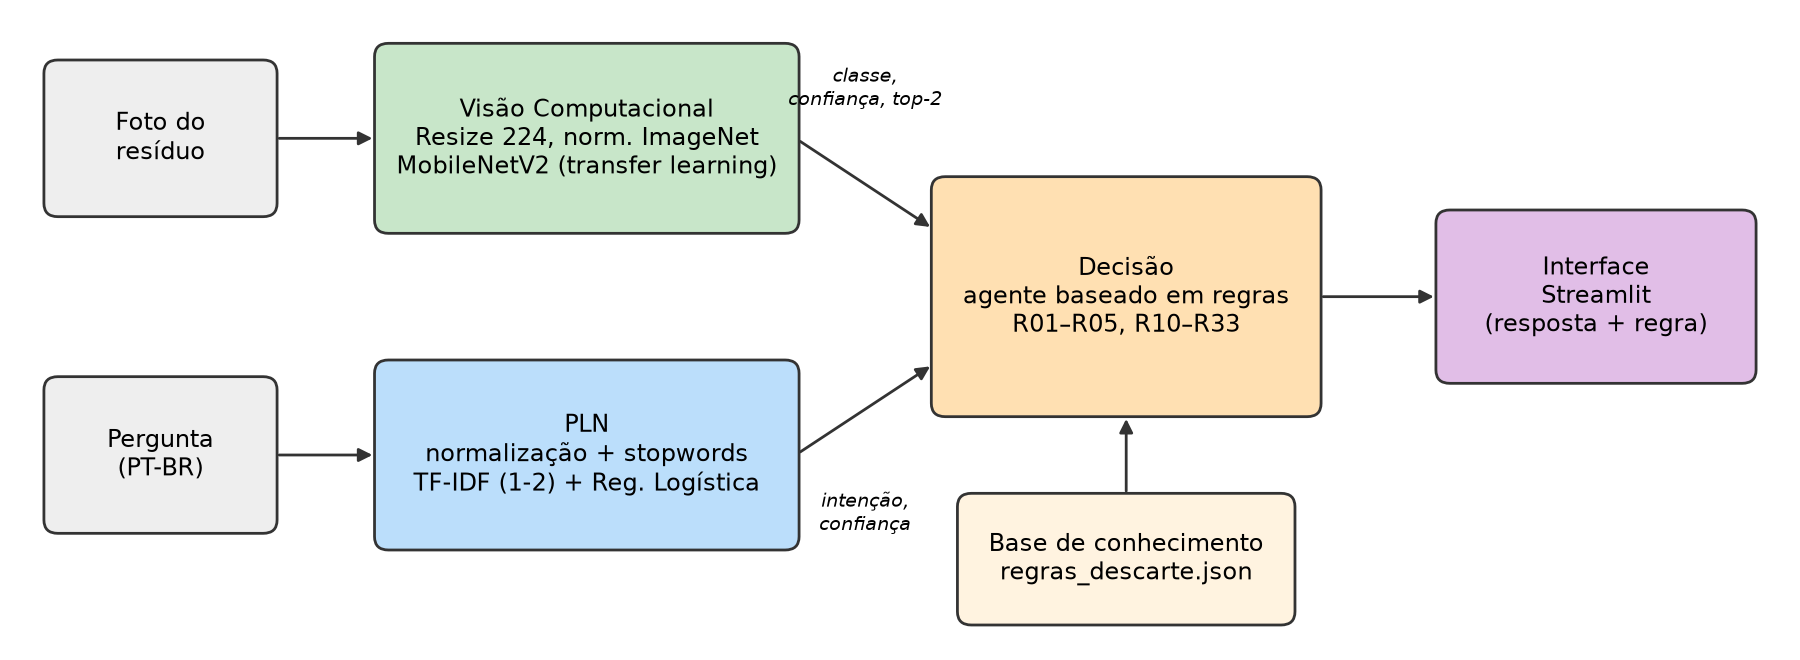
\includegraphics[width=\columnwidth]{arquitetura.png}
\caption{Arquitetura do EcoSort: visão e PLN alimentam o agente baseado em regras.}
\label{fig:arq}
\end{figure}

\subsection{Dados}
\textbf{Imagens.} Utilizou-se a versão redimensionada (512$\times$384) do TrashNet, distribuída sob licença MIT. Foram extraídos apenas os arquivos JPEG das seis pastas de classe, descartando metadados e arquivos não-imagem. O conjunto foi dividido de forma estratificada em treino, validação e teste (70/15/15), resultando em 1.768, 379 e 380 imagens. A classe \emph{trash} é minoritária, com 137 imagens (5,4\%), conforme a Fig.~\ref{fig:dist}.

\begin{figure}[t]
\centering
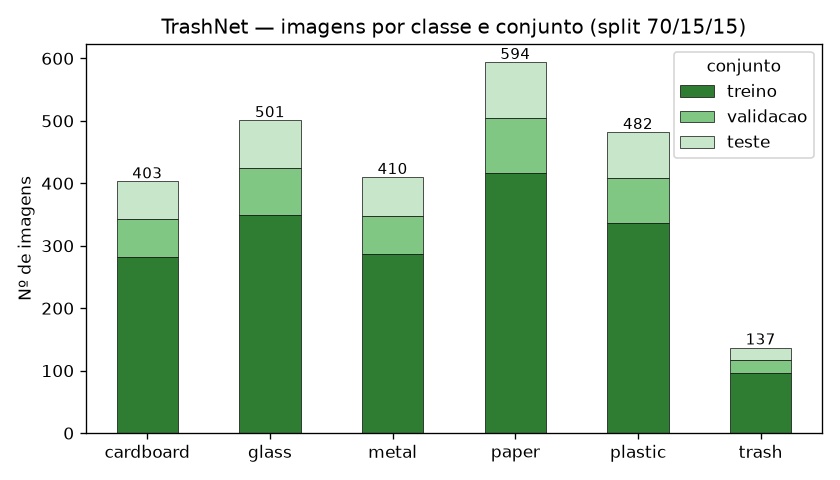
\includegraphics[width=0.92\columnwidth]{dados_distribuicao_classes.png}
\caption{Distribuição das classes do TrashNet por conjunto.}
\label{fig:dist}
\end{figure}

\textbf{Frases.} Como não há corpus público de intenções sobre descarte em português, os autores redigiram 335 frases (65 a 70 por classe; média de 4,5 palavras) em cinco intenções: \emph{como\_descartar}, \emph{e\_reciclavel}, \emph{onde\_levar}, \emph{preparo\_antes} e \emph{fora\_do\_escopo}. O corpus inclui variações informais, abreviações e erros de digitação, além de frases fora do escopo que compartilham vocabulário com o domínio (ex.: ``como lavar roupa branca?''). Não há duplicatas nem dados pessoais. A divisão também foi estratificada em 70/15/15 (234, 50 e 51 frases).

\textbf{Base de conhecimento.} Um arquivo JSON descreve, para cada material, a reciclabilidade, a cor da lixeira segundo a Resolução CONAMA n.º 275/2001 \cite{conama} (papel e papelão: azul; plástico: vermelha; vidro: verde; metal: amarela; rejeito: cinza), instruções de preparo e destinos possíveis.

\subsection{Visão Computacional}
As imagens de treino recebem \emph{data augmentation} (recorte aleatório redimensionado com escala de 0,7 a 1,0, inversões horizontal e vertical, rotação de $\pm15^\circ$ e variação de brilho, contraste e saturação); validação e teste usam redimensionamento para 256 e recorte central de 224$\times$224. Todas as imagens são normalizadas com média e desvio do ImageNet.

O modelo é uma MobileNetV2 pré-treinada no ImageNet, com a camada final substituída por \emph{dropout} (0,3) e uma camada linear de seis saídas, totalizando 2,23 milhões de parâmetros. O treino ocorreu em duas fases: (1) seis épocas com a base congelada, treinando apenas 7.686 parâmetros com AdamW (taxa de aprendizado $10^{-3}$) e mantendo as estatísticas de \emph{batch normalization} do ImageNet; (2) dez épocas de \emph{fine-tuning} dos cinco últimos blocos (1,69 milhão de parâmetros), com taxa de aprendizado $10^{-4}$ na base e $3\times10^{-4}$ na cabeça e decaimento cosseno. A função de perda foi a entropia cruzada com pesos inversamente proporcionais à frequência das classes e \emph{label smoothing} de 0,1. Foi mantido o checkpoint de maior acurácia de validação. Cada época levou cerca de 23~s (fase 1) e 33~s (fase 2) em CPU de oito threads.

\subsection{Processamento de Linguagem Natural}
O pré-processamento converte o texto para minúsculas, remove acentos e pontuação e elimina \emph{stopwords} a partir de uma lista própria. Listas genéricas foram evitadas porque removem termos como ``onde'', ``como'' e ``antes'', que são as pistas mais fortes de intenção neste domínio. Os textos são representados por TF-IDF de unigramas e bigramas com $tf$ sublinear. Compararam-se a Regressão Logística (modelo principal) e o Naive Bayes multinomial (baseline), com o hiperparâmetro de regularização $C$ ou de suavização $\alpha$ escolhido pelo F1 macro na validação. Além do teste, aplicou-se validação cruzada estratificada de cinco partições ao corpus completo, pois o conjunto de teste é pequeno. O modelo implantado foi re-treinado com treino e validação.

\subsection{Componente de Decisão}
O módulo de decisão é um agente reativo cuja percepção é a tupla (classe, confiança da visão, top-2, intenção, confiança do PLN). As regras são avaliadas em ordem de prioridade, e a primeira cuja condição é satisfeita define a ação (Tabela~\ref{tab:regras}). As 24 regras específicas são geradas a partir do produto classe $\times$ intenção, o que garante cobertura completa por construção, verificada por teste automatizado. Os limiares adotados foram 0,35 e 0,6 para a visão e 0,4 para o PLN; o valor 0,4 corresponde ao dobro do acaso para cinco classes. Toda resposta inclui a identificação e a descrição da regra que a gerou.

\begin{table}[t]
\centering
\caption{Regras do agente, em ordem de prioridade}
\label{tab:regras}
\footnotesize
\begin{tabular}{@{}lp{6.4cm}@{}}
\toprule
ID & Condição $\Rightarrow$ ação \\
\midrule
R01 & intenção = fora do escopo e conf.\ PLN $\geq$ 0,4 $\Rightarrow$ explica o escopo \\
R02 & conf.\ visão $<$ 0,35 $\Rightarrow$ pede nova foto \\
R03 & conf.\ visão $<$ 0,6 e top-1 e top-2 com a mesma lixeira $\Rightarrow$ responde pelo grupo comum \\
R04 & conf.\ visão $<$ 0,6 $\Rightarrow$ mostra as duas hipóteses e pede nova foto \\
R05 & conf.\ PLN $<$ 0,4 $\Rightarrow$ resumo geral do material \\
R10--R33 & classe = $X$, intenção = $Y$, conf.\ $\geq$ 0,6 $\Rightarrow$ resposta específica $(X,Y)$ \\
\bottomrule
\end{tabular}
\end{table}

\subsection{Métricas e Testes}
Para ambos os classificadores foram calculados acurácia, precisão, revocação e F1 por classe, F1 macro e matriz de confusão, sempre no conjunto de teste, usado uma única vez. Para o sistema integrado, mediram-se a cobertura (fração de imagens respondidas sem pedir nova foto) e a acurácia nesse subconjunto, em função do limiar. Foram escritos 37 testes automatizados com pytest, abrangendo as saídas de cada módulo, a cobertura das regras e o fluxo ponta a ponta.

% ---------------------------------------------------------------------
\section{Resultados e Discussão}

\subsection{Visão Computacional}
A Fig.~\ref{fig:curvas} mostra as curvas de treino. A fase com base congelada estabilizou a acurácia de validação em torno de 0,79; o \emph{fine-tuning} elevou-a a 0,887 na última época. A Tabela~\ref{tab:visao} resume o desempenho no teste: acurácia de 0,868 e F1 macro de 0,846, bem acima dos resultados originais do TrashNet \cite{trashnet}, o que confirma o benefício do transfer learning. A classe \emph{trash} teve o pior F1 (0,667): é a menor e a mais heterogênea, pois é definida por exclusão.

\begin{figure}[t]
\centering
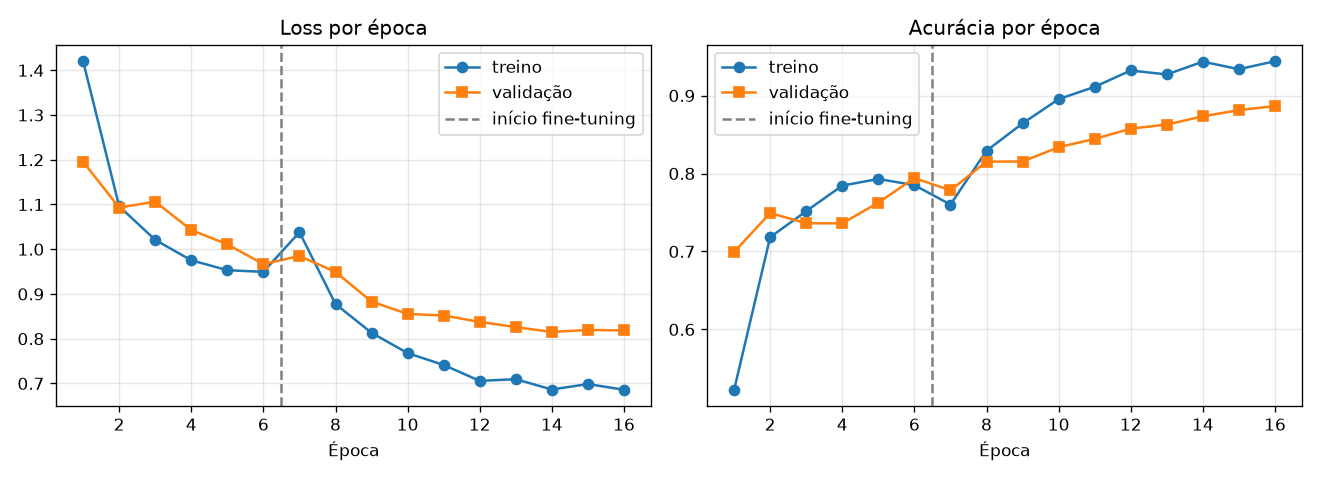
\includegraphics[width=\columnwidth]{visao_curvas_treino.png}
\caption{Loss e acurácia por época. A linha tracejada marca o início do \emph{fine-tuning}.}
\label{fig:curvas}
\end{figure}

\begin{table}[t]
\centering
\caption{Visão: desempenho no conjunto de teste (380 imagens)}
\label{tab:visao}
\footnotesize
\begin{tabular}{@{}lcccc@{}}
\toprule
Classe & Precisão & Revocação & F1 & $n$ \\
\midrule
Papelão (cardboard) & 0,929 & 0,867 & 0,897 & 60 \\
Vidro (glass) & 0,882 & 0,882 & 0,882 & 76 \\
Metal & 0,862 & 0,903 & 0,882 & 62 \\
Papel (paper) & 0,885 & 0,865 & 0,875 & 89 \\
Plástico (plastic) & 0,887 & 0,863 & 0,875 & 73 \\
Rejeito (trash) & 0,600 & 0,750 & 0,667 & 20 \\
\midrule
\multicolumn{5}{@{}l}{Acurácia: 0,868 \quad F1 macro: 0,846} \\
\bottomrule
\end{tabular}
\end{table}

\begin{figure}[t]
\centering
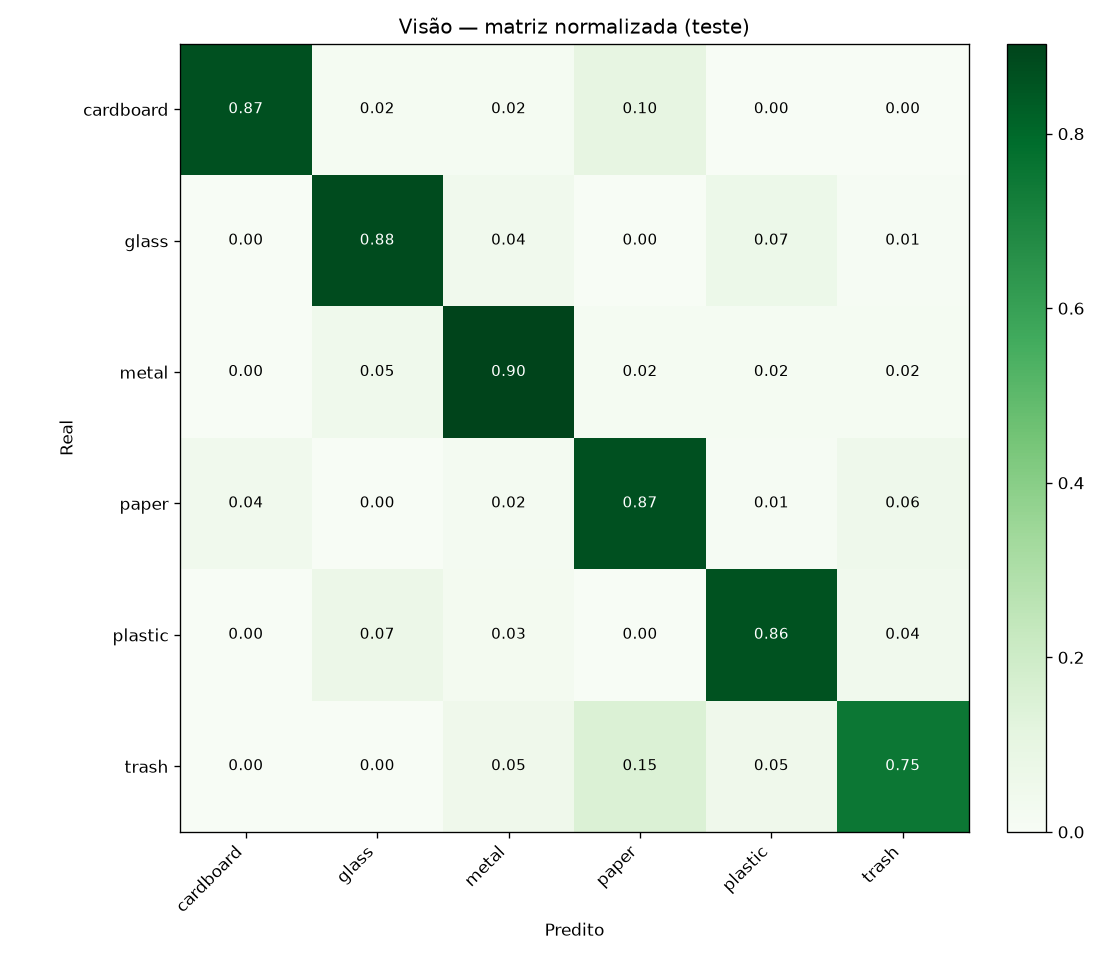
\includegraphics[width=0.85\columnwidth]{visao_matriz_confusao_normalizada.png}
\caption{Matriz de confusão normalizada por linha (teste).}
\label{fig:cm}
\end{figure}

\textbf{Análise de erros.} Dos 50 erros (Fig.~\ref{fig:cm}), os pares mais frequentes foram papelão$\rightarrow$papel (6), vidro$\leftrightarrow$plástico (5 em cada sentido), papel$\rightarrow$rejeito (5) e papel$\rightarrow$papelão (4). Papel e papelão compartilham cor e textura, e a ondulação do papelão desaparece em fotos aproximadas. Garrafas transparentes de vidro e de plástico diferem por pistas sutis, como espessura e brilho, que se perdem na resolução de 224$\times$224. A classe rejeito do TrashNet contém papéis sujos e embalagens laminadas, o que a aproxima visualmente do papel. Os dez erros entre papel e papelão não alteram a lixeira (azul); considerando a lixeira como alvo, a acurácia é de 0,895.

\textbf{Confiança e limiar.} A confiança média foi 0,78 nos acertos e 0,47 nos erros. A Fig.~\ref{fig:limiar} mostra o compromisso entre cobertura e acurácia: com limiar 0,5, a cobertura é de 84,5\% com 95,0\% de acerto; com 0,6, de 76,3\% com 96,6\%; com 0,7, de 64,2\% com 99,2\%. Adotou-se 0,6, que reduz os erros respondidos diretamente de 50 para 10. Desses dez, oito alteram a lixeira; o caso mais grave é uma garrafa de vidro classificada como plástico com confiança 0,83, o que mostra que o limiar não protege contra erros confiantes.

\begin{figure}[t]
\centering
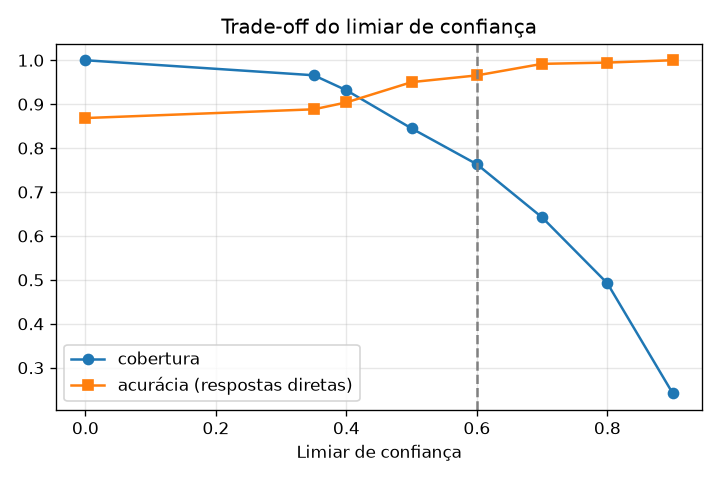
\includegraphics[width=0.85\columnwidth]{limiar_cobertura.png}
\caption{Cobertura e acurácia das respostas diretas em função do limiar.}
\label{fig:limiar}
\end{figure}

\subsection{Processamento de Linguagem Natural}
A Tabela~\ref{tab:pln} compara os modelos. A Regressão Logística ($C=3$) superou o Naive Bayes ($\alpha=0{,}5$) em cerca de dez pontos percentuais tanto no teste quanto na validação cruzada, cujo desvio-padrão (0,047) indica a variância esperada em um corpus pequeno. Por intenção, o F1 da Regressão Logística variou de 1,00 (\emph{preparo\_antes}) a 0,70 (\emph{fora\_do\_escopo}). Dos oito erros no teste, quatro envolvem frases fora do escopo com palavras do domínio: ``quem ganhou o jogo ontem?'' foi classificada como \emph{como\_descartar} devido ao termo ``jogo'' (de ``jogo isso fora''), e ``onde fica o hospital mais próximo?'' como \emph{onde\_levar} devido ao bigrama ``onde fica''. Outros erros decorrem de grafias fora do vocabulário (``recilavel'') e da ambiguidade de ``coleta seletiva'', associada tanto a reciclabilidade quanto a locais de entrega.

\begin{table}[t]
\centering
\caption{PLN: comparação entre modelos}
\label{tab:pln}
\footnotesize
\begin{tabular}{@{}lcccc@{}}
\toprule
 & \multicolumn{2}{c}{Teste (51 frases)} & \multicolumn{2}{c}{Valid. cruzada (5)} \\
Modelo & Acur. & F1 macro & Acur. & F1 macro \\
\midrule
TF-IDF + RL & \textbf{0,843} & \textbf{0,840} & 0,833 $\pm$ 0,047 & 0,830 $\pm$ 0,049 \\
TF-IDF + NB & 0,745 & 0,737 & 0,752 $\pm$ 0,031 & 0,732 $\pm$ 0,038 \\
\bottomrule
\end{tabular}
\end{table}

\subsection{Fluxo Integrado}
Foram registrados 14 casos de ponta a ponta com imagens de teste, disponíveis no repositório. A Tabela~\ref{tab:casos} mostra exemplos representativos. Neles, o componente de decisão evita respostas erradas quando a visão está incerta (R02 e R04), responde com segurança quando as duas hipóteses levam à mesma lixeira, mesmo com confiança de 0,36 (R03), e oferece um resumo quando a pergunta é vaga (R05). O caso de erro confiante (vidro$\rightarrow$plástico) ilustra a principal limitação. Todos os 37 testes automatizados foram aprovados.

\begin{table}[t]
\centering
\caption{Exemplos do fluxo completo (imagens de teste)}
\label{tab:casos}
\scriptsize
\begin{tabular}{@{}p{1.15cm}p{1.9cm}p{1.6cm}p{1.6cm}c@{}}
\toprule
Real & Pergunta & Visão (conf.) & Intenção (conf.) & Regra \\
\midrule
plástico & ``isso é reciclável?'' & plástico (0,99) & e\_reciclavel (0,97) & R27 \\
papel & ``presisa lava antes?'' & papel (0,98) & preparo\_antes (0,69) & R25 \\
vidro & ``como descarto isso?'' & plástico (0,83) & como\_descartar (0,89) & R26$^{*}$ \\
vidro & ``isso é reciclável?'' & vidro (0,598) & e\_reciclavel (0,97) & R04 \\
papel & ``como descarto isso?'' & papelão (0,36) & como\_descartar (0,89) & R03 \\
plástico & ``como descarto isso?'' & plástico (0,29) & como\_descartar (0,89) & R02 \\
metal & ``qual a previsão do tempo hoje?'' & metal (0,87) & fora\_do\_escopo (0,71) & R01 \\
vidro & ``me explica esse item'' & vidro (0,86) & e\_reciclavel (0,33) & R05 \\
\bottomrule
\multicolumn{5}{@{}l}{$^{*}$ Erro da visão com confiança acima do limiar: resposta incorreta.}
\end{tabular}
\end{table}

\subsection{Limitações}
(i) O TrashNet contém fotos com fundo branco, um único objeto e iluminação controlada, de modo que imagens reais tendem a produzir confiança e acurácia menores. (ii) Apenas seis classes são cobertas, sem orgânicos, eletrônicos, pilhas ou embalagens longa-vida. (iii) A confiança é a probabilidade \emph{softmax}, que não foi calibrada. (iv) O PLN baseado em palavras é sensível a erros de digitação e a frases fora do domínio com vocabulário compartilhado, e o corpus é pequeno. (v) Os destinos indicados são genéricos, pois o sistema não usa a localização do usuário.

% ---------------------------------------------------------------------
\section{Conclusão e Trabalhos Futuros}
O EcoSort integra, em um único fluxo funcional, visão computacional, PLN e um agente baseado em regras para orientar o descarte de resíduos. O classificador visual atingiu 86,8\% de acurácia no teste, e o reconhecedor de intenções, 84,3\%, superando o baseline. O componente de decisão mostrou-se essencial, e não apenas acessório: ao tratar a incerteza, elevou a acurácia das respostas diretas para 96,6\%, solicitou nova foto ou apresentou duas hipóteses nos demais casos e tornou cada resposta rastreável a uma regra.

Como trabalhos futuros, propõem-se: coletar fotos reais com fundos variados e novas classes; calibrar a confiança, por exemplo por \emph{temperature scaling}; adotar n-gramas de caracteres ou embeddings de sentenças, como o BERTimbau \cite{bertimbau}, para tornar o PLN mais robusto; e integrar a localização do usuário para indicar pontos de entrega próximos.

% ---------------------------------------------------------------------
\begin{thebibliography}{00}
\bibitem{pnrs} BRASIL, ``Lei n.º 12.305, de 2 de agosto de 2010 --- Institui a Política Nacional de Resíduos Sólidos,'' \emph{Diário Oficial da União}, 2010.
\bibitem{conama} CONAMA, ``Resolução n.º 275, de 25 de abril de 2001 --- Estabelece o código de cores para os diferentes tipos de resíduos,'' \emph{Diário Oficial da União}, 2001.
\bibitem{trashnet} M. Yang and G. Thung, ``Classification of trash for recyclability status,'' CS229 Project Report, Stanford University, 2016.
\bibitem{imagenet} J. Deng, W. Dong, R. Socher, L.-J. Li, K. Li, and L. Fei-Fei, ``ImageNet: A large-scale hierarchical image database,'' in \emph{Proc. IEEE CVPR}, 2009, pp. 248--255.
\bibitem{yosinski} J. Yosinski, J. Clune, Y. Bengio, and H. Lipson, ``How transferable are features in deep neural networks?'' in \emph{Proc. NeurIPS}, 2014, pp. 3320--3328.
\bibitem{mobilenetv2} M. Sandler, A. Howard, M. Zhu, A. Zhmoginov, and L.-C. Chen, ``MobileNetV2: Inverted residuals and linear bottlenecks,'' in \emph{Proc. IEEE CVPR}, 2018, pp. 4510--4520.
\bibitem{wang2012} S. Wang and C. D. Manning, ``Baselines and bigrams: Simple, good sentiment and topic classification,'' in \emph{Proc. ACL}, 2012, pp. 90--94.
\bibitem{russell} S. Russell and P. Norvig, \emph{Artificial Intelligence: A Modern Approach}, 4th ed. Hoboken, NJ: Pearson, 2020.
\bibitem{bertimbau} F. Souza, R. Nogueira, and R. Lotufo, ``BERTimbau: Pretrained BERT models for Brazilian Portuguese,'' in \emph{Proc. BRACIS}, 2020, pp. 403--417.
\bibitem{sklearn} F. Pedregosa \emph{et al.}, ``Scikit-learn: Machine learning in Python,'' \emph{J. Mach. Learn. Res.}, vol. 12, pp. 2825--2830, 2011.
\bibitem{pytorch} A. Paszke \emph{et al.}, ``PyTorch: An imperative style, high-performance deep learning library,'' in \emph{Proc. NeurIPS}, 2019, pp. 8024--8035.
\end{thebibliography}

\end{document}
